\section{Implementation}
\subsection{Information restructuring}


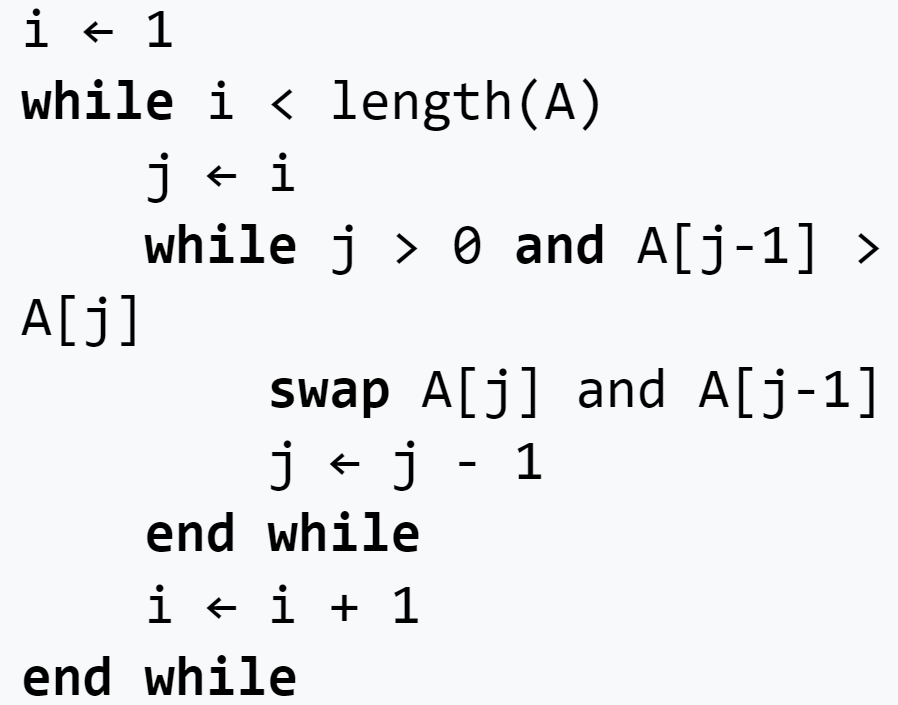
\includegraphics[width=0.35\textwidth]{insertionsort}\par\vspace{0.5cm} %FIX



%code formatting
\begin{lstlisting}
.global _start

.text
_start:
    movl  $4, %eax
    movl  $1, %ebx
    movl  $msg, %ecx
    movl  $len, %edx
    int   $0x80

    movl  $1, %eax
    movl  $0, %ebx
    int   $0x80
.data
msg:
    .ascii  "Hello, world!\n"
    len =   . - msg
\end{lstlisting}
%code formatting

%\hfill \break
%\subsection{Actual Code}
%\subsubsection{Timers}


%\texttt{use\_this}
%{packetTimerMessage}
%\linebreak\texttt{use\_this\_formmating}
%$this-can-also-be-used$

%item formatting
\begin{description}[leftmargin=1em, style=nextline]
\item [\texttt{network\_layer\_allowed\_to\_send}] Signals the network layer that it can send a piece of data.
Here the network layer should make sure the \texttt{from\_network\_layer\_queue}
contains at least one element, after which it can signal \texttt{network\_layer\_ready},
which means that the network layer has prepared at least one element in the queue.

\item [\texttt{network\_layer\_ready}] This signal signals to the link layer that the network layer has prepared an element to be sent in the
  \texttt{from\_network\_layer\_queue} queue and that it should be sent now.

\item [\texttt{data\_for\_network\_layer}]
This signal signals to the network layer that the
\texttt{for\_network\_layer\_queue} contains a data element for it to take care of. (a data element has been received)
\end{description}
%item formatting

\hfill \break
